% Alembic — EMNLP 2026 System Demonstrations submission
%
% Built on the official ACL style files (github.com/acl-org/acl-style-files).
% EMNLP reuses the shared *ACL template; do not modify acl.sty / acl_natbib.bst.
%
% Demo track is SINGLE-BLIND (see https://2026.emnlp.org/calls/demos/):
% authors need not anonymize and self-references are permitted, so we load
% the "preprint" variant (non-anonymous, page numbers, no line numbers).
% Switch to the bare \usepackage{acl} (no options) for the camera-ready copy.
%
% Body text lives in sections/*.tex (one file per section) — edit those,
% not this file, for content changes. This file is preamble + \input wiring.
\documentclass[11pt]{article}
\usepackage[preprint]{acl}

\usepackage{times}
\usepackage{latexsym}
\usepackage[T1]{fontenc}
\usepackage[utf8]{inputenc}
\usepackage{microtype}
\usepackage{inconsolata}
\usepackage{graphicx}
\usepackage{booktabs}
\usepackage{tikz}
\usetikzlibrary{arrows.meta, positioning}

% TODO(authors): fill in the real GitHub URL and screencast link before submission.
\newcommand{\repourl}{https://github.com/aimclub/CoScientist}
\newcommand{\demourl}{TODO-screencast-url}

\title{Alembic: Autonomous Synthesis of MCP Servers from Scientific GitHub Repositories}

% Single-blind review: real author list is permitted at submission time.
\author{
  First Author \\
  ITMO University \\
  \texttt{email@domain} \\\And
  Second Author \\
  ITMO University \\
  \texttt{email@domain} \\
}

\begin{document}
\maketitle

\begin{abstract}
% TODO(authors): tighten to the final ~150 words once numbers are in.
Making a scientific codebase usable by an LLM agent today requires a person to read the repository, resolve its dependencies, and hand-write a tool wrapper around it — a slow step that limits how many of the thousands of published research repositories ever become agent-usable tools. We present \textbf{Alembic}, a system that automates this conversion end to end: given only a GitHub URL, a four-agent pipeline (Explorer, Environment, Coder, Validator, with a Debugger invoked on failure) clones the repository, builds an isolated Python environment, writes a FastMCP server together with a pytest suite, validates every generated tool by actually invoking it, and packages the result as a versioned Docker image exposing a Model Context Protocol (MCP) server over HTTP. No human intervention is required between the URL and a running, tool-tested MCP endpoint. We demonstrate Alembic on repositories spanning cheminformatics, bioinformatics, and signal processing, and compare its design against the two closest systems, ToolMaker and ToolRosella (code2mcp), on environment setup, dependency and external-asset handling, end-to-end validation, and containerized delivery.

\end{abstract}

\section{Introduction}
\label{sec:intro}

Large language model agents are increasingly used to run and combine scientific software, but the software itself is rarely written with agents in mind: a typical research repository assumes a human will read the README, create an environment by hand, and call functions from a Python shell or a bespoke CLI. Turning such a repository into a tool an agent can call reliably — with a stable interface, an isolated environment, and some evidence that it actually works — is a repetitive engineering task that today falls on a person for every repository.

\textbf{Problem and importance.} As the number of scientific repositories that agents are asked to use grows, hand-wrapping each one does not scale. Recent benchmarks confirm that setting up and executing arbitrary research code is itself a hard, largely unsolved agent capability \citep{super2024,corebench2024,astabench2025,researchenvbench2026} — exactly the step Alembic automates. A system that performs this repo-to-tool conversion automatically directly increases the pool of software an agent-based scientific assistant (e.g., a co-scientist system) can draw on, without additional engineering effort per tool.

\textbf{What Alembic does.} Given nothing but a repository URL, Alembic runs a four-stage agent pipeline inside an ephemeral Docker container — \emph{Explorer} (understand the repo), \emph{Environment} (build an installable venv), \emph{Coder} (write a FastMCP server and tests), and \emph{Validator} (prove the server works, calling a \emph{Debugger} sub-agent on failure) — and on success commits the container to a runnable image that serves the generated tools over MCP. Section~\ref{sec:system} describes the pipeline; Section~\ref{sec:demo} describes what a user sees; Section~\ref{sec:related} positions Alembic against the closest prior systems.

\textbf{Novelty.} Unlike systems that require a human-specified target function and invocation example (ToolMaker; \citealp{toolmaker2025}) or that stop at a smoke-tested MCP scaffold on the local filesystem (ToolRosella/code2mcp; \citealp{toolrosella2026}), Alembic (a) discovers the tool surface itself from the repository rather than from a human-authored task spec, and (b) its final artifact is a self-contained, versioned Docker image serving a live MCP endpoint, validated by actually invoking every generated tool rather than only import-checking the generated code. Section~\ref{sec:related} details these differences axis by axis.

\section{System Overview}
\label{sec:system}

\begin{figure}[t]
  \centering
  % TODO(authors): swap for a polished figure if desired; this TikZ diagram
  % compiles as-is and mirrors docs/DESIGN.md's architecture sketch.
  \resizebox{\columnwidth}{!}{%
  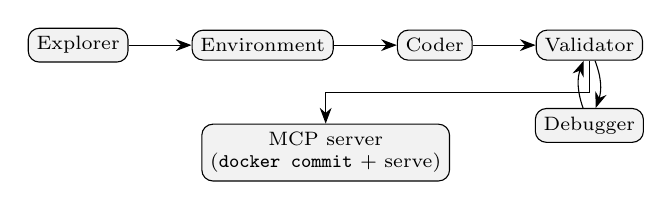
\begin{tikzpicture}[
      node distance=6mm and 8mm,
      stage/.style={draw, rounded corners, fill=black!5, align=center, inner sep=3pt, font=\scriptsize},
      >={Stealth[length=2mm]}
    ]
    \node[stage] (explorer) {Explorer};
    \node[stage, right=of explorer] (env) {Environment};
    \node[stage, right=of env] (coder) {Coder};
    \node[stage, right=of coder] (validator) {Validator};
    \node[stage, below=of validator] (debugger) {Debugger};
    \node[stage, below=8mm of env, xshift=8mm] (serve) {MCP server\\(\texttt{docker commit} + serve)};

    \draw[->] (explorer) -- (env);
    \draw[->] (env) -- (coder);
    \draw[->] (coder) -- (validator);
    \draw[->] (validator) edge[bend left=20] (debugger);
    \draw[->] (debugger) edge[bend left=20] (validator);
    \draw[->] (validator.south) -- ++(0,-4mm) -| (serve.north);
  \end{tikzpicture}%
  }
  \caption{Alembic pipeline: four sequential agents run inside a build container, with a Debugger sub-agent invoked on failure; on success the container is committed and re-launched as an MCP server.}
  \label{fig:pipeline}
\end{figure}

Alembic is built on Google's Agent Development Kit (ADK) and LiteLLM, so all agents share one configurable underlying model. The four stages communicate only through markdown hand-off reports (\texttt{reports/*.md}) written to a shared working directory — there is no shared chat history across agents — which keeps each agent's context focused on its own sub-task and makes intermediate state inspectable.

\paragraph{Explorer.} Clones the repository, reads the README and a small budget of key files (setup/packaging files, entry-point scripts, configs), and writes a report describing the repository's purpose, its environment requirements, and one to five candidate MCP tool usage scenarios with concrete example inputs.

\paragraph{Environment.} Builds an isolated environment satisfying the repository's declared dependencies, falling back across strategies (\texttt{uv}, pip, conda, \texttt{apt-get} for system libraries) and, for repositories requiring an older Python than the server itself, maintaining two separate virtual environments. A compatibility check replays the repository's own imports inside the built environment to catch version conflicts before code generation starts.

\paragraph{Coder.} Reads the Explorer's report, verifies the real function signatures it plans to wrap by inspecting the source, and generates a FastMCP server plus a pytest suite. Each generated tool shells out to the repository's own environment rather than re-implementing repository logic, which keeps the generated wrapper thin and keeps correctness tied to the original code.

\paragraph{Validator (+ Debugger).} Statically checks the generated server, runs the generated test suite, and then \emph{actually invokes every generated tool} against the sample inputs from the hand-off report — catching runtime faults (missing binaries, missing dependencies, argument-parsing bugs) that a mocked unit test cannot. On failure, a Debugger sub-agent classifies the failure (missing binary, missing package, code bug, or unrecoverable environment fault) and fixes only that class before the Validator re-checks, bounded by a small retry budget.

On success, the build container is committed to a versioned image and re-launched in \emph{serve} mode, exposing the generated tools as an MCP server over \texttt{streamable-http}.

\section{Demonstration}
\label{sec:demo}

\paragraph{Target audience.} Alembic targets two groups: (i) engineers building agent-based scientific assistants who need a growing library of callable tools without hand-writing a wrapper per repository, and (ii) maintainers of scientific software who want a low-effort path to making their tool agent-accessible.

\paragraph{Functionality shown in the demo.} A single command,
\begin{quote}
\small\texttt{start\_chain.py <repo-url>}
\end{quote}
takes a public GitHub URL and produces a running MCP server; the screencast (Section~\ref{sec:availability}) shows this end to end on a real scientific repository, including the generated server code, the validation report, and a live tool call against the resulting MCP endpoint from an MCP client. We also show the \texttt{--resume <stage>} flag, which restarts the pipeline from any stage while preserving prior artifacts, and a batch mode (\texttt{run\_benchmark.py}) that runs the pipeline over many repositories in parallel and reports per-repository success.

\section{Comparison with Existing Systems}
\label{sec:related}

Two recent systems address closely related problems. \textbf{ToolMaker} \citep{toolmaker2025} converts a repository into a single Python function given a human-authored task specification (target function name, argument list, and one example invocation), then closes an iterative implement–run–diagnose–rewrite loop around that one function inside a reproducible, \texttt{install.sh}-built Docker image. \textbf{ToolRosella} \citep{toolrosella2026} (its \texttt{code2mcp} component) is closest in output format: a LangGraph pipeline that statically analyzes a repository, generates an MCP scaffold, and repairs it through a review–revise–fix loop driven by traceback analysis, but validation stops at import-level smoke testing and the artifact is a local folder rather than a container image.

Table~\ref{tab:comparison} summarizes the key differences.

\begin{table*}[t]
  \centering
  \small
  \begin{tabular}{@{}p{2.3cm}p{4cm}p{4cm}p{4cm}@{}}
    \toprule
    & \textbf{ToolMaker} & \textbf{ToolRosella} & \textbf{Alembic} \\
    \midrule
    Tool surface & human-specified, single function & auto-discovered, capped list & auto-discovered, 1--5 tools \\
    Environment strategy & single global pip install & uv $\to$ conda $\to$ venv & uv/venv, two-venv fallback \\
    End-to-end validation & LLM judge on 1 example & import smoke test only & live invocation, every tool \\
    Repair loop & implement--diagnose--rewrite ($\le$30) & review--revise--fix ($\le$5) & debugger sub-agent ($\le$2/tool) \\
    Delivered artifact & reproducible Docker image, in-container function & local folder (\texttt{mcp\_output/}) & versioned Docker image, live MCP server \\
    \bottomrule
  \end{tabular}
  \caption{Alembic against the two closest repo-to-tool systems. See Appendix~\ref{sec:appendix-comparison} for the full axis-by-axis comparison.}
  \label{tab:comparison}
\end{table*}

The systems are complementary rather than strictly ordered: ToolMaker's task-specified, single-function setup buys stronger correctness guarantees (held-out unit tests, an LLM judge) at the cost of requiring a human to specify the target signature per tool, which is a different point on the autonomy/verifiability trade-off than Alembic's fully autonomous, multi-tool discovery.

\section{Availability}
\label{sec:availability}

Alembic is released under the MIT license at \url{\repourl}. A screencast demonstrating the full pipeline on a real repository is available at \url{\demourl}. % TODO(authors): unlisted YouTube link or MPEG4 supplementary file, \(\le\) 2.5 minutes.

\section*{Evaluation}
% TODO(authors): EMNLP demo submissions without any reported evaluation risk desk
% rejection (see https://2026.emnlp.org/calls/demos/). Replace this placeholder
% with the actual benchmark table (per-repo success across the four pipeline
% stages, e.g. the output of run_benchmark.py) before submitting.
We evaluate Alembic on a benchmark of public scientific repositories spanning cheminformatics, bioinformatics, and signal processing, run end to end with \texttt{run\_benchmark.py}. For each repository we report whether the environment build, code generation, and validation stages succeeded, and the fraction of generated tools that pass live invocation. \textit{[TODO: insert the benchmark table and headline success rate once the run completes.]}

\section*{Limitations}
Alembic's Coder stage wraps a repository's existing entry points rather than reasoning about undocumented internal APIs, so repositories with no clear callable surface (e.g., research code only runnable as an end-to-end script with hard-coded paths) yield fewer or coarser-grained tools. The Environment stage's fallback chain (\texttt{uv} $\to$ pip $\to$ conda $\to$ \texttt{apt-get}) is not guaranteed to resolve every dependency conflict, and repositories requiring GPU-specific builds or proprietary system libraries may fail environment setup outright. Validation invokes each tool with a small set of sample inputs derived from the Explorer's report rather than held-out test cases, so it can catch execution failures but does not verify semantic correctness of tool outputs the way a held-out unit-test suite would.

\input{sections/ethics}
\input{sections/acknowledgments}

\bibliography{custom}

\appendix
\section{Full System-Comparison Table}
\label{sec:appendix-comparison}
% TODO(authors): trim docs/TOOLMAKER_COMPARISON.md and docs/TOOLROSELLA_COMPARISON.md
% down to fit the 2-page appendix limit for the demo track.
Extended, axis-by-axis comparison against ToolMaker and ToolRosella (secret/API-key handling, external asset downloads, tool-count control, and containerization depth), summarized from \texttt{docs/TOOLMAKER\_COMPARISON.md} and \texttt{docs/TOOLROSELLA\_COMPARISON.md} in the project repository.


\end{document}
